\subsection{CONNECTED SUBSETS OF R}

THEOREM 4. A subset A of R is connected if and only if A is an interval. 1) The condition is necessary. Suppose that A is connected: if A consists of a single point, it is an interval. If A has more than one

point, let \(a\) and \(b\) be two points of A such that \(a < b\) ; by Proposition 1 of no. 4 it is enough to show that every \(x\) such that \(a < x < b\) belongs to A. Now, if \(x \notin A\) we should have \(A \subset \mathbb{C}\{x\}\) ; but \(\mathbb{C}\{x\}\) is the union of two disjoint open sets \([] \leftarrow, x[\) and \(]x, \rightarrow[\) , each of which meets A, and therefore A would not be connected, contrary to hypothesis. 2) The condition is sufficient. Let us show first that every compact interval \([a, b]\) is connected. For each integer \(n > 0\) , let \(V_{1/n}\) be the entourage consisting of all pairs \((x, y)\) such that \(|x - y| \leqslant 1/n\) ; by Proposition 6 of Chapter II, § 4, no. 4, it is enough to show that every pair of points \(x, y\) of \([a, b]\) can be joined by a \(V_{1/n}\) -chain. Let \(p\) be the greatest integer such that \(p/n \leqslant x\) and let \(q\) be the greatest integer such that \(q/n \leqslant y\) ( \(p\) and \(q\) exist by reason of Theorem 1 of no. 1); then \(p \leqslant q\) . If \(p = q\) then \(y - x < 1/n\) and the points \(x\) and \(y\) form a \(V_{1/n}\) -chain. If \(q > p\) , put \(x_i = (p + i)/n\) ( \(i = 1, 2, \ldots, q - p\) ); we have \(x_1 - x \leqslant 1/n\) , \(y - x_{q-p} \leqslant 1/n\) and \(x_{i+1} - x_i = 1/n\) , hence the points \(x, x_1, x_2, \ldots, x_{q-p}, y\) form a \(V_{1/n}\) -chain joining \(x\) and \(y\) .

If now I is any interval not consisting of a single point, and if \(a\) and \(b\) are any two points of I such that \(a < b\) , then the interval \([a, b]\) is contained in I and is connected, and hence I is connected.

COROLLARY I. The real line is a connected and locally connected space.

COROLLARY 2. The only compact connected subsets of R are the bounded closed intervals.

By Theorem 4, a subset of R which does not contain any interval consisting of more than one point is totally disconnected; this is true, for example, of the set Q of rational numbers, since the set \(\mathbb{Q}\) of irrational numbers is dense in R.

PROPOSITION 2. Every non-empty open set in R is the union of a countable family of mutually disjoint open intervals.

Let A be a non-empty open set in R. Since R is locally connected, every component of A is a connected open set (Chapter I, § 11, no. 6, Proposition 11) and therefore an open interval by Theorem 4. Any two of these open intervals are disjoint; on the other hand, each of them contains a rational number; hence the set of these intervals has a power less than or equal to that of Q, i.e.~is countable.

It follows that every closed set in R is the complement of the union of a (finite or infinite) sequence \((I_{n})\) of mutually disjoint open intervals. These intervals are said to be contiguous to the closed set under consideration. Conversely, given such a sequence of intervals, the complement of their union is a closed set to which these intervals are contiguous.

Example. Let us define by induction a countable family \((I_{n,p})\) of mutually disjoint open intervals as follows:

The integer \(n\) takes all values \(\geqslant 0\) , and for each value of \(n, p\) takes the values \(1, 2, 3, \ldots, 2^n\) . All the intervals \(I_{n,p}\) are contained in

\[
\mathbf {A} = [ \mathbf {0}, \mathbf {1} ],
\]

and we take \(\mathbf{I}_{0,1} = ]1/3, 2/3[\) (the ``middle third'' of {]}0, 1{[}). Suppose now that the \(2^{m+1} - 1\) intervals \(\mathbf{I}_{n,p}\) have been defined for \(0 \leqslant n \leqslant m\) in such a way that, if \(\mathbf{J}_m\) is their union, the set \(\mathbf{A} \cap \complement_{\mathbf{J}_m}\) is the union of \(2^{m+1}\) mutually disjoint closed intervals \(\mathbf{K}_{m,p}\) ( \(1 \leqslant p \leqslant 2^{m+1}\) ) each of length \(\frac{1}{3^{m+1}}\) . If \(\mathbf{K}_{m,p} = [a, b]\) we then take \(\mathbf{I}_{m+1,p}\) to be the open interval \(\left]a + \frac{b - a}{3}, b - \frac{b - a}{3}\right[\) (the ``middle third'' of the interval {]}a, b{[}), and it is immediately verified that the induction can continue in this way (Fig. 3).

\pandocbounded{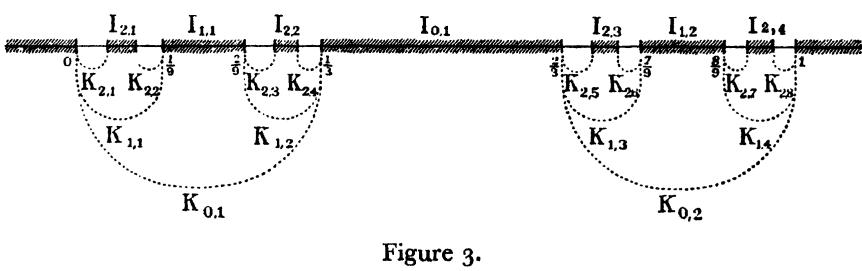
\includegraphics[keepaspectratio]{images/part002_c6c4994f.jpg}}\\
Figure 3.
If \(\mathbf{K}'\) is the complement of the union of the \(\mathbf{I}_{n,p}\) , the closed set \(\mathbf{K} = \mathbf{A} \cap \mathbf{K}'\) is called Cantor's triadic set. Clearly \(\mathbf{K}\) is compact (no. 2, Theorem 2); also \(\mathbf{K}\) is totally disconnected. For if \(\mathbf{K}\) contained an interval I of length \(>0\) , then I would be contained in some interval \(\mathbf{K}_{m,p}\) ; hence its length would be \(\leqslant 1/3^{m+1}\) for each \(m\) , which is absurd.

